\def \Qa % 1
{
\begin{textarea}[]
	\only<1>{
		\centering
		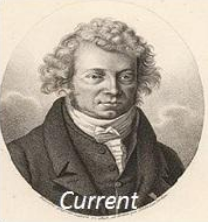
\includegraphics[width=0.4\textwidth]{../categories/media/SIunits/AndreMarieAmpere.png}
	}
	\only<2>{
		Who is Andr\'{e}-Marie Amp\`{e}re?
	}
\end{textarea}
}


\def \Qb % 2
{
\begin{textarea}[]
	\only<1>{
		\centering
		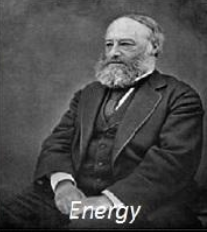
\includegraphics[width=0.4\textwidth]{../categories/media/SIunits/JamesJoule.png}
	}
	\only<2>{
		Who is James Joule?
	}
\end{textarea}
}

\def \Qc % 2
{
\begin{textarea}[]
	\only<1>{
		\centering
		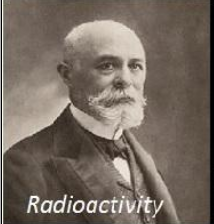
\includegraphics[width=0.4\textwidth]{../categories/media/SIunits/HenriBecquerel.png}
	}
	\only<2>{
		Who is Henri Becquerel?
	}
\end{textarea}
}

\def \Qd % 3
{
\begin{textarea}[]
	\only<1>{
		\centering
		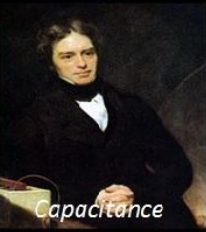
\includegraphics[width=0.4\textwidth]{../categories/media/SIunits/MichaelFaraday.png}
	}
	\only<2>{
		Who is Michael Faraday?
	}
\end{textarea}
}

\def \Qe % 4
{
\begin{textarea}[]
	\only<1>{
		\centering
		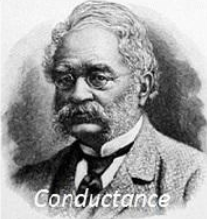
\includegraphics[width=0.4\textwidth]{../categories/media/SIunits/WernerVonSiemens.png}
	}
	\only<2>{
		Who is Werner von Siemens?
	}
\end{textarea}
}
